\section{Kasutajaliides}
Vastavalt peatükile \ref{analysis_interface_subsection} kasutajaliidese realiseerimise tehnoloogiaks
on valitud React.Js raamistik.

Kasutajaliidese rakendus koosneb \textit{React JSX.Element} komponentidest ja teenustest.
Komponendid tagavad rakendusele nõutud funktsionaalsust ja välimust ning teenused vahendavad andmeid komponentide 
ja serveriosa vahel.

Rakenduse koosseisus on palju erinevaid komponente, suurem osa nendest on lihtsamad komponendid või tavalised
CRUD-loogikaga komponendid, mistõttu ei ole nende realiseerimise käesolevas peatükis eraldi kirjeldatud. Koodibaas
täismahus on vaadatav  Lisas X oleva viitega koodi repositooriumile. Käesolevas peatükis kirjeldatakse vaid mõned
komponendid, mis infosüsteemi äriloogika seisukohalt vajavad kompleksset ülesehitust ja funktsionaalsust -- 
ehitusmaterjali lisamise vorm ja kalkulaator.

Materjali loomiseks ja redigeerimiseks on luuakse vorm, mis täidab samaaegselt mõlemat rolli.
Kui vormi avamisel oli antud ehitusmaterjali ID, siis laetakse vastav materjal andmebaasist redigeerimiseks, 
vastasel juhul vormi avamisel luuakse serveriosale päringuga uus materjal mustandi staatusega, mida hakatakse
vormis redigeerima. Materjali vorm koosneb kahest React komponendist - vormi põhi ja materjali omaduse plokk.
Vormi põhi on suurem komponent \textit{MaterialForm.tsx}, mille kaudu redigeeritakse materjali staatilised 
väljad:

\begin{itemize}
    \item nimetus (\textit{title}) -- tekstiväli,
    \item materjali tüüp (\textit{materialCategoryId}) -- valiklist materjalide kategooriatest, 
    \item tootja (\textit{manufacturerId}) -- valiklist materjalide tootjatest,
    \item allikas (\textit{source}) -- tekstiväli,
    \item viide allikale (\textit{link}) -- tekstiväli,
    \item kommentaar (\textit{comment}) -- tekstiväli.
\end{itemize}

Materjalide omaduste (nt tihedus, soojusjuhtivus) arv on muutuv -- mõne materjali puhul võivad olla salvestatud
kõik omadused, teise materjali puhul vaid mõned neist. Lisaks sellele, tulevikus võib infosüsteemile olla lisatud
võimalus salvestada muud omadused, mis on tarvis teiste arvutuste jaoks. Sellest tingituna peab olema võimalus kuvada
ja redigeerida need omadused, mis on materjali puhul määratud. Lisaks peavad olema näidatud ka omadused,
mida on võimalik lisaks määrata. Materjali omadusi redigeerimiseks tehakse väiksem taaskasutatav 
komponent \textit{MaterialPropertyCard.tsx}. Komponendil on järgmised väljad:
\begin{itemize}
    \item väärtus (\textit{value}) -- materjali omaduse arvuline väärtus,
    \item tõendatud (\textit{verified}) -- boolean väärtus,
    \item allikas (\textit{source}) -- tekstiväli.
\end{itemize}

Põhikomponendis on redigeeritava materjali puhul eksisteerivad omadused on salvestatud vormi oleku objektis \textit{materjal.materialProperties}
listi kujul. Iga omaduse jaoks luuakse iteratiivselt vastav komponent \textit{MaterialPropertyCard}, millele antakse omaduse objekt ja funktsioon, 
mis töötleb sisendi andmete muutmist ja tagastab põhikomponendisse sisestatud väärtused. Põhikomponendis uuendatakse olekut ja vastavalt
saadetakse ka päringuid materjali uuendamiseks andmebaasis. Komponendil \textit{MaterialPropertyCard} välimuse seisukohalt on kaks olekut sõltuvalt 
sellest, kas 
\begin{itemize}
    \item vastav omadus on materjalile lisatud
    \item vastav omadus ei ole materjalile lisatud, kuid seda on võimalik lisada.  
\end{itemize}

Materjali omaduste komponentide välimus mõlemas olekus on näidatud Joonisel \ref{fig:development_frontend_propertycard}.
 \begin{figure}[ht]
    \centering
    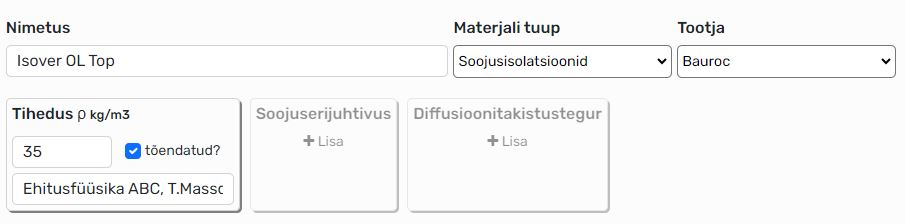
\includegraphics[width=1\textwidth]{figures/development/frontend_propertycard.JPG}
    \caption[\textit{PropertyCard} materjali omaduste komponendid materjali vormis]{\textit{PropertyCard.tsx komponendid materjali vormis}}
    \label{fig:development_frontend_propertycard}
\end{figure}

Infosüsteemi teine oluline ning keerulisema loogikaga osa on kalkulaator. Kalkulaator koosneb järgmistest plokkidest:
\begin{itemize}
    \item arvutuse seadistuste osa, milles valitakse arvutuse parameetrid (sisemine ja välimine keskkonnad, konstruktsiooni tüüp);
    \item konstruktsiooni kihtide plokk, milles lisatakse konstruktsioonile kihte ja valitakse kihtide omadused (materjal, paksus);
    \item tulemuste esitamise plokk, milles graafiliselt esitatakse konstruktsiooni kihtide skemaatilist joonist, graafikuid ning arvuline tulemus 
    (soojusjuhtivus U ja veeaurutakistus Zp).
\end{itemize}

Kalkulaatori põhiline \textit{React} komponent on \textit{Therm.tsx}. Komponent juhib ja korraldab alluvate komponentide tööd. Komponendis on mitu oleku (\textit{state}) objekti:
\begin{itemize}
    \item \textit{optionsLibrary} -- objekt, mis hoiab arvutuse parameetrite valikud (keskkonnad, konstruktsioonitüübid),
    \item \textit{materials} -- objekt, mis hoiab materjale, mida kasutatakse konstruktsiooni kihtide mudeldamisel,
    \item \textit{calculationData} -- objekt, mis hoiab arvutuse lähteandmeid, mida edastatakse serverile
    \item \textit{calculationResult} -- objekt, mis hoiab serverilt tulnud arvutuse tulemused.
\end{itemize}

Ülaltoodud objektide loomiseks kasutatakse  sisseehitatud lahendust \textit{UseState}, mille abil loob React juhitavat oleku objekti. \textit{UseState}
objektide eelis on oleku muutuste jälgimine ning kõikide olekust sõltuvate komponentide automaatne uuendamine oleku muutmisel.

Kalkulaatori põhikomponent koosneb väiksematest komponentidest, mis oma funktsionaalsusest lähtuvalt vastavad varem nimetatud kalkulaatori plokkidele.
Kalkulaatori alamkomponendid on:
\begin{itemize}
    \item \textit{ThermOptions.tsx} -- komponendile antakse arvutuse parameetrite andmeobjekt, arvutuse lähteandete objekt ning funktsioon kasutajasisendi töötluseks;
    sisendi muutmisel tagastab komponent põhikomponendisse sisendi uut väärtust, millega uuendatakse arvutuse lähteandmete objekti.
    \item \textit{LayersBlock.tsx} -- komponendile antakse edasi ehitusmaterialide andmeobjekt, mida kasutatakse konstruktsiooni kihtide lisamise vormis, ning funktsiooni
    konstruktsiooni kihtide salvestamiseks; komponent on kompleksse ülesehitusega ja omakorda omab struktuuris alamkomponente; komponent tagastab põhikomponendisse konstruktsiooni
    kihtide listi;
    \item \textit{ResultBlock.tsx} -- komponendile antakse kihtide plokis koostatud kihtide objekt ning serverilt tulnud arvutuse tulemused graafikute joonestamiseks. 
\end{itemize}

\textit{Therm.tsx} komponendi struktuur on toodud Joonisel \ref{fig:development_frontend_therm}.
\begin{figure}[ht]
    \centering
    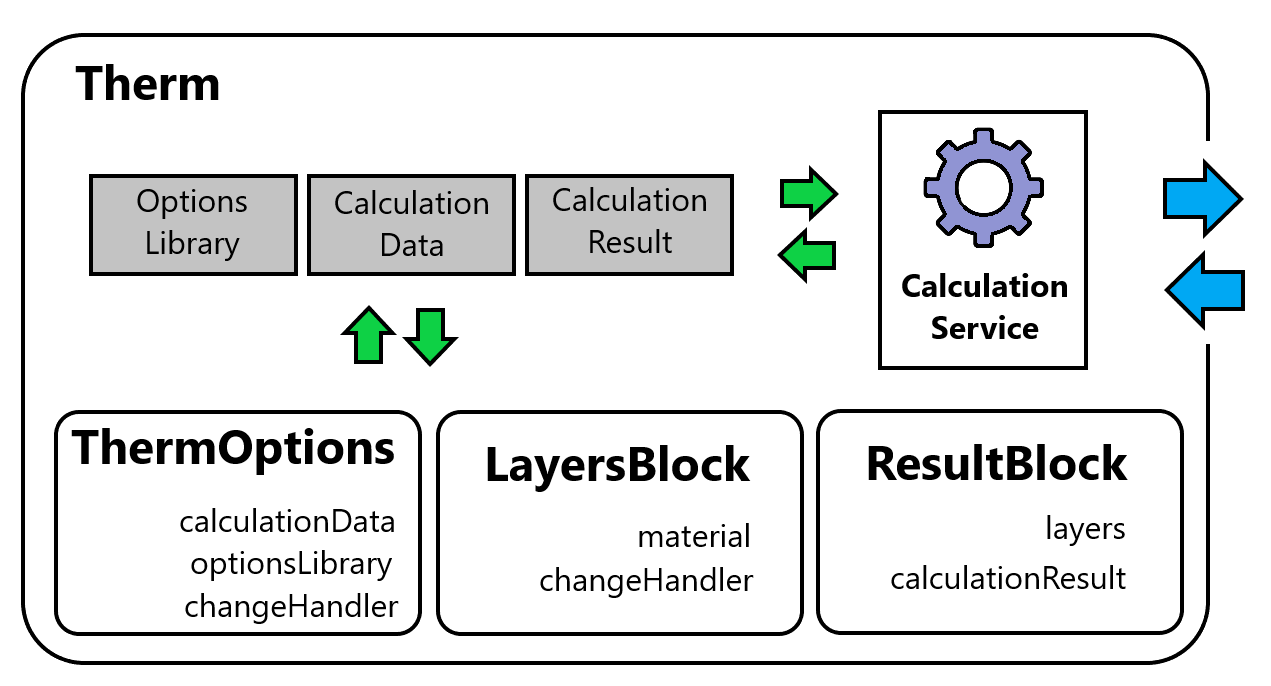
\includegraphics[width=.8\textwidth]{figures/development/frontend_term_structure.png}
    \caption[Kasutajaliidese komponendi \textit{Therm.tsx} struktuur]{\textit{Therm.tsx komponendi struktuur}}
    \label{fig:development_frontend_therm}
\end{figure}

Alamkomponentide loogika on piiratud oma vastutusalaga, kõik alamkomponendid on üks teisest sõltumatud ning on juhitud põhikomponendist. Serveriosaga suhtlemine toimub põhikomponendis
oleva teenuse kaudu (\textit{CalculationService}). Põhikomponent küsib teenuse kaudu serveriosalt andmeid, mis on tarvis kalkulaatoris olevate valiklistide täitmiseks ja komplekteerib
kasutajas isendist andmeobjekti, mille struktuur vastab serveriosa vastavale liidesele. Samuti komponent saadab serverile päringut arvutuse lähteandmetega ning 
töötleb ja edastab vastust tulemuste esitamise komponendile.

Konstruktsiooni kihtide modelleerimisega tegeleb kihtide plokk \textit{LayersBlock.tsx} (Joonis \ref{fig:dev_frontend_layersblock}). Komponent kujutab ennast konstruktsiooni kihtide
nimekirja koos uue kihi lisamise ja olemasolevate kihtide redigeerimise vormidega. Rakenduse äriloogika eeldab, et kasutajal peab olema võimalus kihtide järjekorda muuta, seetõttu
on nimekiri tehtud dünaamilise nimekirjana, mille puhul saab kasutaja elementide asukohta muuta. Igal nimekirja real on ees ikoon, mille haarates saab kihti tõmmata õigesse kohta. 


\begin{figure}[ht]
    \centering
    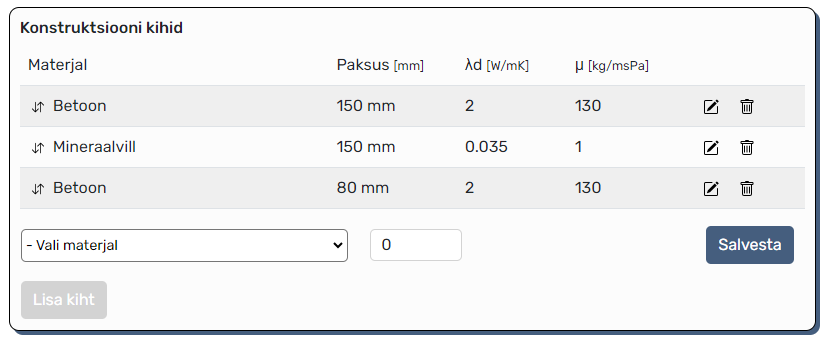
\includegraphics[width=1\textwidth]{figures/development/frontennd_layersblock.png}
    \caption[LayersBlock.tsx -- konstruktsiooni kihtide modeleerimine]{\textit{LayersBlock.tsx -- konstruktsiooni kihtide modeleerimine}}
    \label{fig:dev_frontend_layersblock}
\end{figure}


Tulemuste esitamise komponent \textit{ResultBlock.tsx} tegeleb tulemuste representeerimisega graafilisel viisil: joonestatakse lihtsustatud kujul mudeldatud konstruktsiooni skeemi, 
mille peale kantakse serverilt tulnud andmete põhjal temperatuuri ja veeaururõhkude graafiku jooned. Nõutud funktsionaalsus on otstarbekas lahendada HTML5 \textit{canvas} elemendiga, mis
on ette nähtud kahemõõtmeliste piltide genereerimiseks; element on manipuleeritav \textit{JavaScript} keelega. 

Konstruktsiooni skemaatilise joonise koostamiseks on lähteandmeteks konstruktsiooni kihtide objekt (list). Igas kihis sisaldub teave, mis on tarvis joonise koostamiseks: 
kihi paksus (väljendatud millimeetrites), kihi materjal koos materjali kategooriaga. 
Konstruktsiooni kihtide paksustest arvutatakse proportsionaalsed väärtused \textit{canvas} elemendil kuvamiseks. Iga kihi lisamisega arvutatakse proportsioonid uuesti - kihtide arvu
ja vastavalt konstruktsiooni kogupaksuse suurendamisega muutub mõõtkava väiksemaks. Kihtide värvilise täide tegemiseks võetakse värvi kood materjali kategoorias salvestatud koodist.
Materjali kategooriate värvikoode saab kasutaja vastaval rakenduse lehel redigeerida. 
\dots

\begin{figure}[ht]
    \centering
    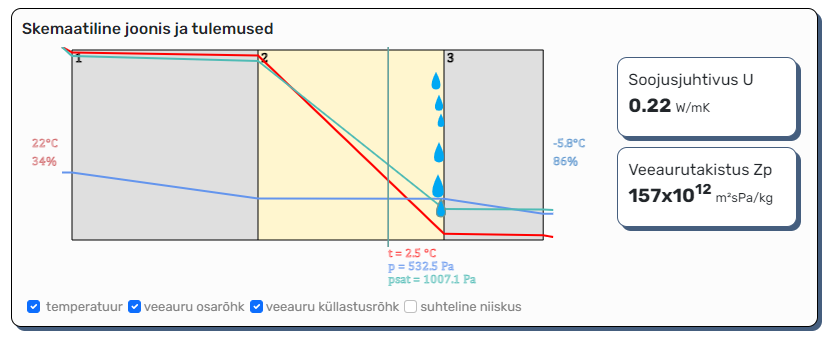
\includegraphics[width=1\textwidth]{figures/development/frontennd_resultblock.png}
    \caption[ResultBlock.tsx -- tulemuste esitamise plokk]{\textit{ResultBlock.tsx -- tulemuste esitamise plokk}}
    \label{fig:development_frontend_results}
\end{figure}


